\chapter{MACworkflow}

\begin{figure}[ht!]
\centering
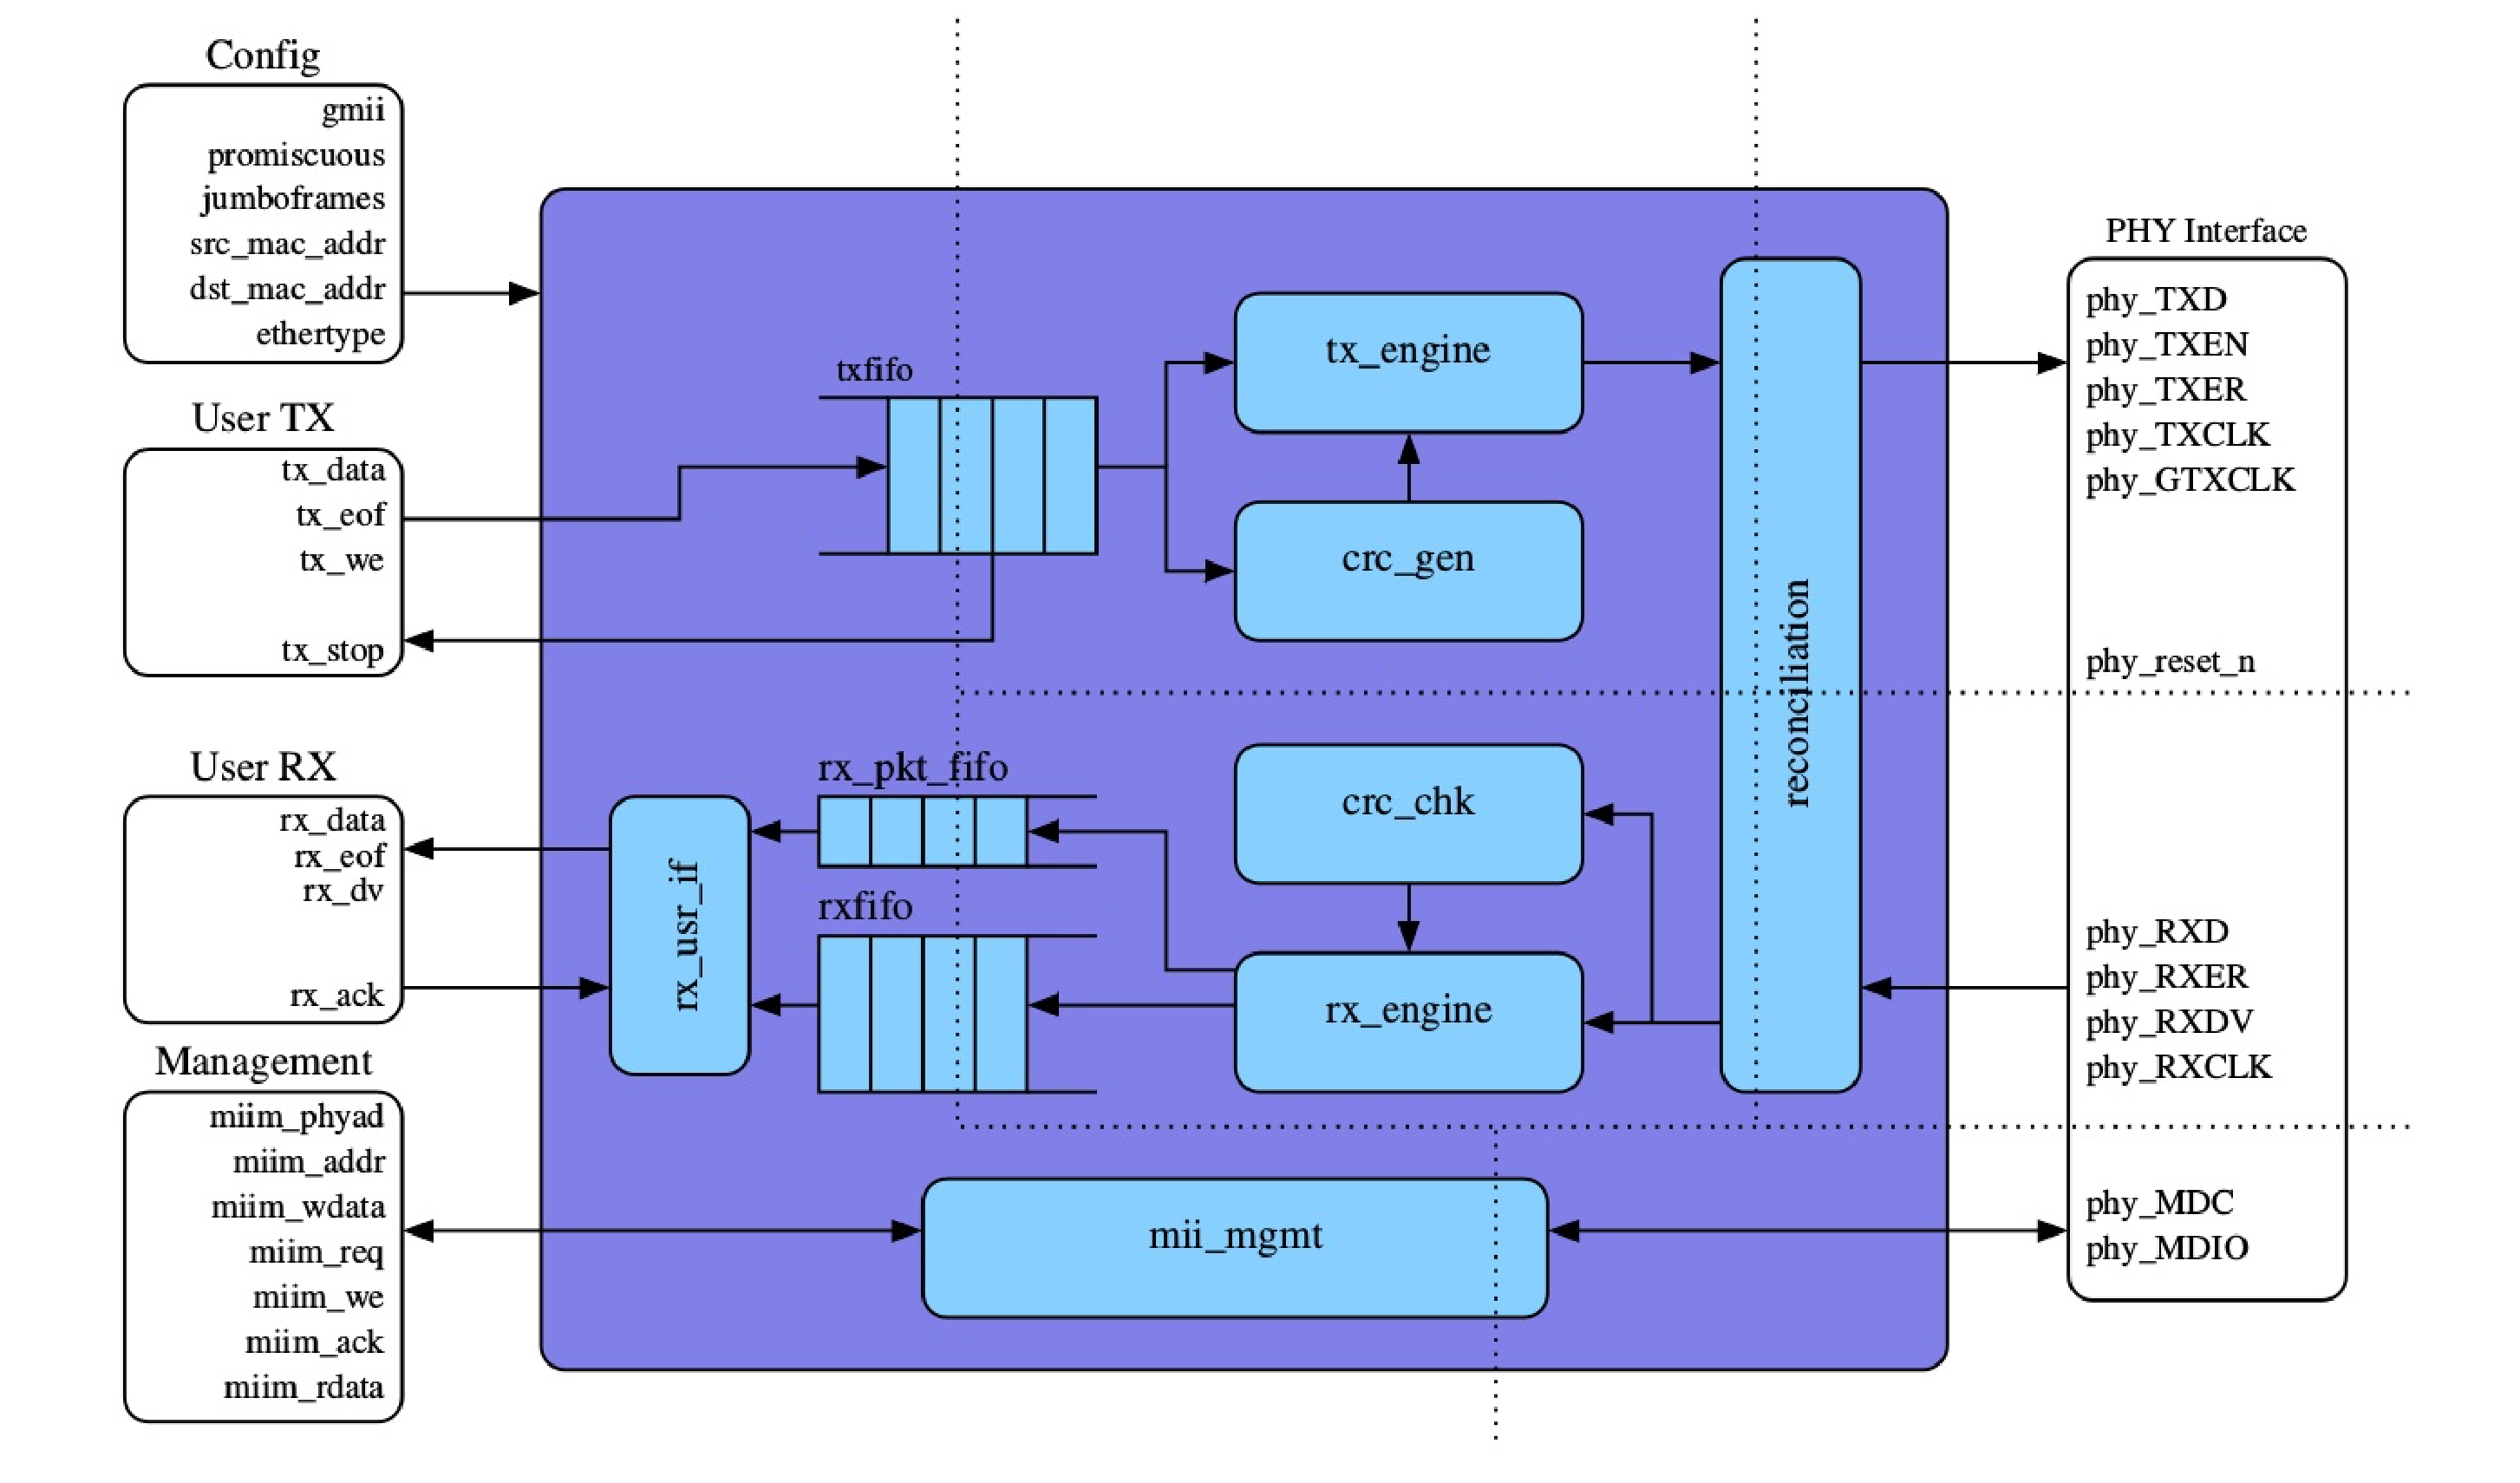
\includegraphics[scale=0.25]{eps/mac10.eps}
\caption{The mac10}
\label{mac10}
\end{figure}

This is the block diagram of the MAC core, which is very important in understanding how the MAC functions.

From the MAC chapter, we know that the MAC mainly has three parts: reception, reconciliation, and transmission.

The transmission part includes txfifo, $tx_engine$, and $crc_gen$, which takes the user data and send it to reconciliation module, which send it to ethernet phy.

The reception part includes $rx_usr_if$, $rx_pkt_fifo$, $rxfifo$, $rx_engine$, and $crc_chk$, which takes data from reconciliation, throwing away bad frames, and then present them to the user

The reconciliation part deals with GMII interface to phy.

TO use the MAC core, we can simply implement the configuration ports that MAC presents to us, which is listed and explained as follows:

gmii: a flag that indicates whether the MAC core should be communicate with the phy in GMII mode or MII mode.

promiscous: a flag that indicates the MAC core should filter incoming packages to those with destination of $src_mac_addr$

$src_mac_addr$: this is the MAC address to use as the source of transmitted ethernet frames and the filter for what received frames to not discard when not in promiscous mode

$dst_mac_addr$: this is the MAC address to use as the destination of transmitted ethernet frames.

ethertype: the EtherType/Length field for outgoing packets

ifg: this is the number of cycles inserted between packets, should be $>= 0x0D$




